\documentclass[letterpaper, 12 pt, conference]{ieeeconf}  % 
\usepackage{graphicx}
\usepackage{url}
\usepackage{hyperref}

\title{\LARGE \bf Genetic Algorithm}

\author{Minqi Xu   20845758   m259xu@uwaterloo.ca % <-this % stops a space
\thanks{Minqi Xu  are with the 
 School of Computer Science, University of Waterloo,
200 University Avenue, Waterloo, Ontario, Canada N2L 3G1.        {\tt\small }}%
}


\begin{document}
\onecolumn
\maketitle
%
\begin{abstract}
The main purpose of this report is to briefly introduce genetic algorithms. The report will mention the relationship between this algorithm and natural selection. Then, the report will mention which scenarios the genetic algorithm is suitable for and why it will give a high-quality solution. And finally, the genetic algorithm will be applied to a specific problem, the Travelling Salesman Problem (TSP), which is a common problem in the field of computer science, and show how the problem is solved based on the genetic algorithm. And its result.
\end{abstract}
%

\section{Introduction}
\label{sec:intro}
% Citation examples: \cite{An82,An09,Go89,Ra10}.
Genetic algorithms (GAs) are stochastic approaches based on biological evolutionary processes proposed by Holland in 1975.\cite{Ho75} It is inspired by the process of natural selection and evolution. The most basic point is that the fittest individuals are more likely to survive and reproduce; therefore, the next generation is more likely to be better than the previous generation. By continuously iterating the generation, the population trends become better. More details will be provided in the next section.


\section{Related Work}
\label{sec:rw}
In 1859, Charles Darwin proposed his theory of evolution by natural selection as an explanation for adaption and speciation, He defined natural selection as the "principle by which each slight variation (of a trait), if useful, is preserved". \cite{Cd59} In Charles Darwin's autobiography, published in 1958, Darwin realized that "favourable variations would tend to be preserved, and unfavourable ones to be destroyed. The result of this would be the formation of new species". \cite{Cd58} From these points, we can summarize the core idea of natural selection. The first point is that variation is the result of genetic differences which can arise through mutation or genetic recombination. Here mutation is the change in the structure of the DNA which is used to make up genes. The second point is offspring inherit traits from their parents. The third point is overproduction, which means it is possible that children can be better than their parents. Forth point is environment is challenging, and individuals need to struggle to survive. The fifth point is stated as "Survival of the fittest", which means that the individuals who own advantageous traits are more likely to survive and reproduce so that advantageous traits are more likely to pass to the next generation. The last point is over time and generation iterations, the frequency of advantageous traits will increase in the population.

Meta-heuristics are general algorithmic frameworks, often nature-inspired, designed to solve complex optimization problems. \cite{Lb08}. And GAs are iterative stochastic optimization meta-heuristics that mimic the natural evolution process. Each candidate solution of an optimization problem (which will be mentioned later in this section) is represented as an individual in a pool that constitutes a GA population. A solution (individual) is characterized by the number of genes, which are sometimes organized in chromosomes. Depending on its fitness value, a single individual is selected for proliferation and subjected to the genetic operators - typically selection, crossover, and mutation. The application of these operators results in the next generation of solutions whose average fitness is ideally better than that in the previous generation. The fitness value of an individual reflects the level of achieving the optimization goal given the corresponding solution, which is provided by the fitness function. The fitness function encodes optimization goals and evaluates how well those goals are achieved during execution. \cite{Dp14}

In computer science, the optimization problem is the problem of finding the best solution from all feasible solutions. \cite{wikiop} And Travelling Salesman Problem (TSP) is one of the most famous benchmarks, significant, historic, and very hard combinatorial optimization problems. \cite{Ah17} It is documented by Euler in 1759, whose interest was in solving the knight's tour problem. \cite{Pl99} TSP is stated as given a list of cities and the distance between each pair of cities, what is the shortest possible route that visits each city exactly once and returns to the origin city? It is said to be an NP-hard problem, which means no efficient way to find the optimal solution to the problem since the number of potential answers grows factorially. For example, if we only have 10 cities, then there are $\frac{9!}{2}=181440$ potential solutions with fixing the starting city. Compared to traditional methods like brute force (traverse every possible solution, and find the optimal one), GAs are capable of efficiently searching large solution spaces. Instead of exploring every possible solution, they narrowed the search to promising regions of the solution space using a guided and evolutionary process.


\section{Algorithm Implementation}
\label{sec:rw}
In this section, we will apply GAs on TSP as an example to explain GAs.

We will define some terms first to facilitate explanation in the subsequent steps. A gene in the GAs corresponds to a city (vertex) in TSP. Individual (chromosome) corresponds to a single walk satisfied the condition which is every vertex only appears once in the walk except the starting vertex appears at the end of the walk again. Note that in graph theory, a walk defines as a sequence of alternating vertices and edges, but here, we only take the vertices part, and edges can be implied by the order of vertices. A parent corresponds to two individuals that will combine to produce new individual(s). Mating Pool corresponds to the collection of parents. Fitness corresponds to a function that tells us how good the individual is.

The first step of the algorithm is initiation. After importing data, we need to randomly generate individuals (with random order of vertices). And collect all randomly generated individuals as our initial generation. Then apply the fitness function to every individual in the initial generation. The Fitness function of this problem can be defined as the inverse of the length of the walk. The shorter routes receive higher fitness scores, indicating a higher chance of being selected for the next generation.

The second step of the algorithm is selection. This process is akin to "survival of the fittest". Individuals with higher fitness scores have a higher probability of being selected for reproduction. We have already calculated the fitness of each individual, then we can sort based on it. After sorting, we will apply the selection method to the current generation. But at the same time, we are going to use a technique called elitism, which allows the best individuals from the current generation to be directly carried into the next generation. This guarantees that the solution quality obtained by the GAs will not decrease from one generation to the next one.\cite{Bs22} Which can let the algorithm converge faster. So we will introduce a hyper-parameter called the elite\_size to control the number of individuals we want to carry to the next generation. Then we will select the rest of the selected individuals based on the selection method. Here we will provide two selection methods. The first one is called the fitness proportionate selection (roulette wheel selection). In fitness proportionate selection, the fitness function assigns a fitness to possible solutions or chromosomes. This fitness score is used to associate a probability of selection with each individual chromosome. For example, if $f_i$ is the fitness of individual $i$ in the population, its probability of being selected is $p_i=\frac{f_i}{F}$ where $F$ is the sum of the fitness of all individuals in the population. \cite{wikifps} Another selection method is called stochastic universal sampling (SUS). It is a development of fitness proportionate selection which exhibits no bias and minimal spread. SUS uses a single random value to sample all of the solutions by choosing them at evenly spaced intervals. It performs better when there exists an individual with an extremely large fitness compared to others. \cite{wikisus} It is an optimal sequential sampling algorithm with no bias, minimal spread, and achieves all N samples in a single traversal. The following is a code fragment for SUS. \cite{Jeb}
\begin{verbatim}
    ptr = rand()
    for (sum=i=0; i<N; i++)
        for (sum += ExpVal[i]; sum > ptr; ptr++)
            selectInd(i)
\end{verbatim}

The third step of the algorithm is crossover. This is the process of combining genetic information from two individuals (as parents) to create new offspring. Firstly, we need to pair sampled individuals and generate the mating pool. After that, we can apply the crossover operator on the mating pool. Here, we will provide two crossover operators. The first operator is called partially mapped crossover. It is proposed by Goldberg and Lingle.\cite{Dgrl85} We need to choose two random cut points on parents to build offspring, and the fragment between cut points, one parent's string is mapped onto the other parent's string, and the remaining information is exchanged. For example, the cut points are marked with $``|"$. $P_1=(348|271|65)$ and $P_2=(425|168|37)$. The mapping sections are between two cut points. In this example, $2\leftrightarrow 1,7\leftrightarrow 6, 1\leftrightarrow 8$. Two mapping sections are copied with each other to make offspring as $O_1=(xxx|168|xx)$ and $O_2=(xxx|271|xx)$. Then we can fill further bits (from original parents), for those which have no conflict as $O_1=(34x|168|x5)$ and $O_2=(4x5|271|3x)$. The first $x$ in $O_1$ is 8 which comes from the first parent but 8 is already in $O_1$, again, 1 exists in $O_1$, so we need to check mapping $2\leftrightarrow 1$, so 2 occupies at first $x$. Similarly, the second $x$ comes from $7\leftrightarrow 6$, and 7 occupies the second $x$. Therefore, $O_1=(342|168|75)$, similarly, $O_2=(485|271|36)$. \cite{Ah17} Another operator is called the cycle crossover. The cycle crossover operator was first proposed by Oliver et al. \cite{Imo87}. Using this technique to create offspring in such a way that each bit with its position comes from one of the parents. For example, given two individuals as parents: $P_1=(12345678)$ and $P_2=(85213647)$. Now it is up to us to choose the first bit for the offspring to be either from the first or the second parent. Here, the first bit of the offspring has to be 1 or 8, let us choose it to be 1: $O_1=(1xxxxxxx)$. Now every bit in the offspring should be taken from one of its parents with the same position, which means that we have no choice, the next bit to be considered is 8, as the bit from the second parent at the same selected position is 8. So we have to choose 8 from the first parent, thus $O_1=(1xxxxxx8)$. This turnout implies bit 7 because of a similar reason, $O_1=(1xxxxx78)$. Next, put 4 at the 4th position as $O_1=(1xx4xx78)$. After this, 1 comes which is already in the list, and one cycle is completed. Then we need to fill the remaining blank positions with the bits of those positions which are in the second parent: $O_1=(15243678)$. \cite{Ah17}

After crossover, we are moving to the last key process of the genetic algorithm, which is called mutation. Mutation introduces small random changes to the offspring, thereby maintaining diversity in the population. In TSP, we can simply swap two vertices' positions in a walk. In this step, we will introduce another hyper-parameter called mutation rate, which controls the probability that an individual mutates. We can traverse every point on the walk, doing a test based on the mutation rate each time, if it passes, randomly swap the current vertex with another vertex in the walk.

Then repeating selection, crossover, and mutation until the termination criteria are reached. Usually, the termination criteria include the maximum number of generations, finding a satisfactory solution, or running out of computation resources. 


\section{Results and Discussion}
The following results are the genetic algorithm of different selection methods and crossover operators applied to a TSP of 38 cities.\cite{Uwtsp} The population size for each generation is set to 100, elite size is set to 20, mutation rate is set to 0.01, number of generations is set to 5000. And given that the optimal walk is of length 6656.
\begin{figure}[h!]
    \centering
    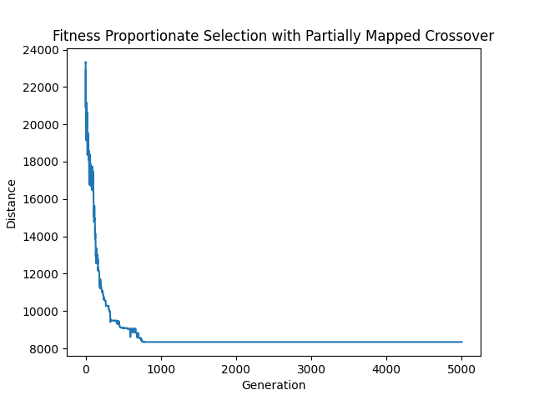
\includegraphics{project-style-files/ga1.png}
\end{figure}
\begin{figure}[h!]
    \centering
    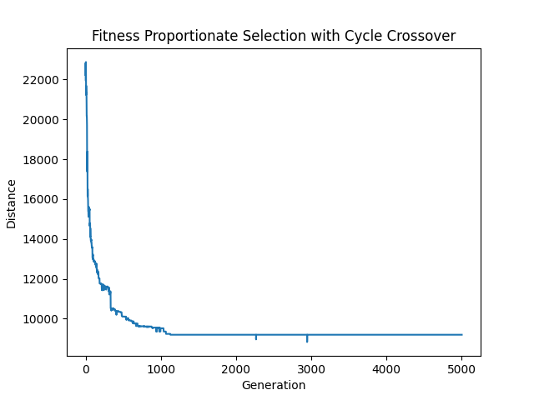
\includegraphics{project-style-files/ga2.png}
\end{figure}
\begin{figure}[h!]
    \centering
    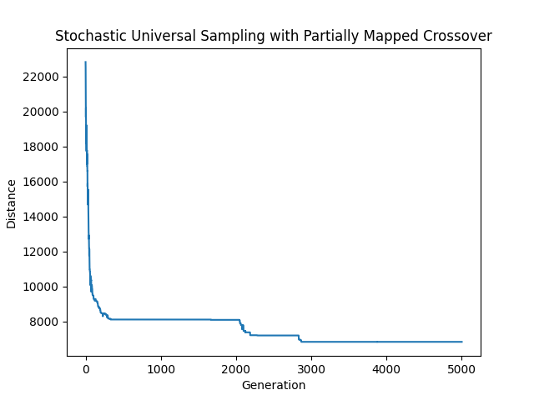
\includegraphics{project-style-files/ga3.png}
\end{figure}
\begin{figure}[h!]
    \centering
    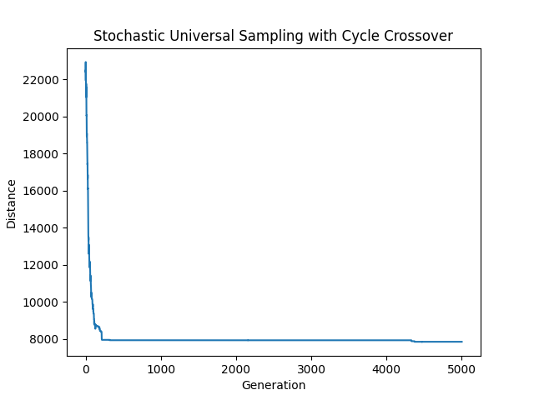
\includegraphics{project-style-files/ga4.png}
\end{figure}
\newpage
\hfill\break
Generally speaking, the results of the genetic algorithm are reasonably high-quality, and the solutions are relatively close to the optimal solution. And it is fortunately that one of the solutions produced by SUS and Partially Mapped Crossover is really close to the optimal solution when it is close to 3000 generations.


\section{Benefits and shortcomings of the GAs}
\label{sec:rw}
Genetic algorithm has several advantages. It does the global search, which means it is able to explore diverse regions of the solution space and find global optima or near-optimal solutions. It can also adapt the changing problem landscapes and constraints, which is able to solve dynamic optimization problems.

However, there are some shortcomings. Repeated fitness function evaluations for complex problems are usually the most constrained part of artificial evolutionary algorithms. Finding the optimal solution to complex high-dimensional, multi-modal problems often requires very expensive fitness function evaluations. Also, the convergence speed may be relatively slow, especially for complex or high-dimensional problems due to a large search space size. In many problems, GAs tends to converge towards local optima or even arbitrary points rather than the global optimum of the problem. This means that it does not know how to sacrifice short-term fitness to gain longer-term fitness. And it is also difficult to operate on a dynamic data set since the chromosomes converge very early on to a solution that may no longer be valid for later data. \cite{wikiga}

\section{Conclusion}

Genetic algorithms have proven to be powerful and versatile optimization techniques, capable of tackling complex problems like the TSP. Through the example of applying GAs on TSP, it is shown their ability to find near-optimal solutions. Although GAs have certain limitations, there are many ways to solve some of the limitations, so they are still valuable tools in various real-world applications and research fields. Following are examples of ways to solve the limitations, divide a complex problem into smaller problems to reduce the complexity, increase the probability of mutation or improved the fitness function to solve the local optimum of the convergence value, by increasing genetic diversity and preventing early convergence, or by increasing the probability of mutation when solution quality drops (this is called triggering hypermutation), or by occasionally introducing entirely new, randomly generated elements into the gene pool (this is called random migration) to solve the problem of dynamic dataset.\cite{wikiga}

\newpage
\bibliographystyle{IEEEbib}
\bibliography{template}

\end{document}



